\chapter{Results}
\label{chap:results}
In this chapter we present the results of this research. In Section \ref{section:results:results_optimization} we present the optimized parameters $(r_1,b_1,r_2,b_2)$ for the non-amplified and amplified LSH schemes for different configuration settings for $n$ and $t$. This allows us to perform an in-depth analysis of the conditions under which amplification adds value. The results of the bootstrap evaluation can be found in the next two Section. First, we present a comparison of MinHash with FSS in Section \ref{section:results:MinHash_vs_FSS}. Then, we examine how the amplified and non-amplified LSH schemes hold up against each other in Section \ref{section:results:amplified_vs_non_amplified}.

\section{Optimization of parameters of (amplified) LSH scheme}
\label{section:results:results_optimization}
In this section we delve into the results of the optimization of the function $z(r_1,b_1,r_2,b_2| w_{FP}, w_{FN})))$ with respect to $(r_1,b_1,r_2,b_2)$ in Equation \ref{eq:optimization_amplified} using Algorithm \ref{alg:optimize_lsh_paramaters}, with $w_{FP} = w_{FN} = 0.5$. This is a worthwile exercise not only because we need the optimized values of ($r_1^{opt},b_1^{opt},r_2^{opt},b_2^{opt}$) to use in the experimental application of the schemes to the data, but also because such a theoretical analysis of optimality of conditions for amplification has not been undertaken before. 

\begin{table}
    \centering
    \caption[Results of optimization of $\hat{z}$]{\textbf{Results of optimization of $\hat{z}$}. For the combinations of parameters $(n,t)\in \{16,32,64,128,256,512,1024\} \times \{0.1,0.5,0.8\}$ we give the optimal parameters and optimal value of $\hat{z}$ in the amplified setting and non-amplified setting. $n$ refer to the size of the sketch. $t$ denotes the similarity threshold value at which entities should be regarded as duplicates by the LSH scheme. The last column gives the \% decrease of $\hat{z}$ in the amplified setting compared to the non-amplified setting}
    \begin{tabular}{l|l|l|l|l|l|l}
        \multicolumn{1}{c}{} & \multicolumn{1}{c}{}  & \multicolumn{2}{c}{Not amplified (one layer)} & \multicolumn{2}{c}{Amplified (two layers)}  & \\
        \hline
        \multicolumn{1}{c}{$n$} & \multicolumn{1}{c}{$t$} & \multicolumn{1}{c}{($r_1^{opt},b_1^{opt},r_2^{opt},b_2^{opt}$)} & \multicolumn{1}{c}{$\hat{z}$} & \multicolumn{1}{c}{($r_1^{opt},b_1^{opt},r_2^{opt},b_2^{opt}$)} & $\hat{z}$ &  \% change $\hat{z}$      \\
        \hline
        16 & 0.1 & (1,15,1,1) & 0.03033 & (1,1,1,15) & 0.03033 & 0\%  \\
        32 & 0.1& (1,17,1,1) & 0.03033 & (1,16,2,1) & 0.02501& -17.54\%  \\
        64 & 0.1& (1,33,1,1)& 0.03033 & (1,4,2,8) & 0.02137&  -29.55\%  \\
        128 & 0.1 & (2,64,1,1) & 0.02290 & (1,16,4,2)  & 0.01752& -23.47\% \\
        256 & 0.1 & (2,117,1,1) & 0.01929 & (1,12,5,2) & 0.01451 & -24.75\% \\
        512 & 0.1 & (2,117,1,1) & 0.01929 & (1,16,8,4) & 0.01178 & -38.90\% \\
        1024 & 0.1 & (2,117,1,1) & 0.01929 & (1,18,11,5) & 0.00992 & -48.55\% \\
        \hline
        16 & 0.5 & (3,5,1,1) & 0.06824 & (1,2,4,2) & 0.06553 & -3.97\%  \\
        32 & 0.5& (4,8,1,1) & 0.05884 & (1,2,5,3) & 0.05588& -5.03\%  \\
        64 & 0.5& (4,14,1,1)& 0.05250 & (2,4,4,2) & 0.04607&  -12.24\%  \\
        128 & 0.5 & (5,25,1,1) & 0.04374 &  (2,3,4,5) & 0.03843& -12.13\% \\
        256 & 0.5 & (6,42,1,1) & 0.03805 & (2,7,9,2) & 0.0307 & -19.17\% \\
        512 & 0.5 & (7,73,1,1) & 0.03402 & (2,7,12,3) & 0.02545 & -25.19\% \\
        1024 & 0.5 & (8,128,1,1) & 0.03111 & (2,6,12,7) & 0.02104  & -32.35\% \\
        \hline
        16 & 0.8 & (8,2,1,1) & 0.04680 & (4,2,2,1) & 0.04627 &-1.13\%  \\
        32 & 0.8& (10,3,1,1) & 0.04108 & (5,3,2,1) & 0.04006 & -2.48\%  \\
        64 & 0.8& (10,6,1,1)& 0.03500 & (4,2,4,2) & 0.03257 &  -6.52\%  \\
        128 & 0.8 & (11,5,1,1) & 0.02939 &  (7,6,3,1) & 0.02648 & -9.62\% \\
        256 & 0.8 & (13,9,1,1)) & 0.02494 & (5,4,6,2) & 0.02197 & -11.89\% \\
        512 & 0.8 & (18,28,1,1) & 0.02181 & (6,6,7,2) & 0.01795 & -17.70\% \\
        1024 & 0.8 & (20,51,1,1) & 0.01915 & (8,9,7,2) & 0.01485  & -22.45\% \\


        \end{tabular}
\label{table:optimized_paramaters_results}
\end{table}

Since the total number of LSH configurations evaluated equals $228$, we only show a subset of the results. These can be found in Table \ref{table:optimized_paramaters_results}, where we include all optimization results related to the threshold values $t \in (0.1,0.5,0.8)$. These threshold values have been chosen so that we can compare results for a relatively small threshold, a relatively large threshold, and a threshold value in between. By zooming in on both relatively small and large thresholds, we are able to optimally draw insights and conclusions on the theoretical added value of the amplification schemes for varying types of LSH applications. For each threshold $t$ we show the optimized structure ($r_1^{opt},b_1^{opt},r_2^{opt},b_2^{opt}$) for the non-amplified scheme in column $3$ and for the amplified scheme in column $5$. Column $4$ and $6$ contain the optimal values of $z(\cdot)$, from now on referred to as $\hat{z}$, for the non-amplified and amplified scheme, respectively. The last column of the table shows the relatively percentage decrease in $\hat{z}$ when one switches from a non-amplified scheme to an amplified scheme for the specified configuration $(n,t)$.

First, we look at the optimal structures of the schemes. We find that the amplified scheme almost always delivers a theoretically superior result. Among the $21$ examples listed in the table, there is only one configuration of hyperparameters, namely $n=16$ and $t=0.1$, where the theoretically optimal structure of the non-amplified and amplified scheme is exactly the same. In all other cases a set-up with two layers should be preferred for users that aim to minimize the chance of false negative and false positives.

But that is not the only theoretical property that users in general care about. It is also important that the extraction of candidate pairs is not too computationally expensive, so that the scalability of the scheme is guaranteed. One of the key factors with respect to the speed of extracting candidate pairs is the size of $r_1$. If $r_1$ is small, two effects occur that increase the number of operations of the candidate extraction algorithm as specified Algorithm in \ref{alg:extract_candidate_pairs_amplified}. The first effect is that there is a higher chance in each band of the first layer that inputs $p$ and $p'$ hash to the same key. Secondly, we need to visit more bands in the first stage of the structure to find potential candidate pairs. 

For an amplified scheme to deliver better results with respect to the chance of false negative and false positives, a change in the structure compared to the non-amplified scheme is required. Hence, we need $r_2 * b_2 > 1$, which, keeping the number of hash functions $n$ the same, implies that either $r_1$ or $b_1$ (or both) becomes smaller in the amplified version. In practice, we find that both parameters tend to be smaller in the optimal amplified strucutre. For very small thresholds, such as $t=0.1$, we consistently find that $r_1^{opt} = 1$ in the optimal amplified strucutre. While $r_1^{opt} = 1$ for relatively small values of $n$ in the non-amplified structure as well, $r_1^{opt} = 2$ for $n=1024$. This implies that there are about $2$ as many bands in the amplified structure for $n=1024$ and $t=0.1$, with each band due to its smaller size guaranteed to produce more candidate pairs. Both of these factors decrease the efficiency of the algorithm for extracting candidate pairs and thus hamper its scalability. For larger thresholds, the influence of $r_1^{opt}$ on the scalability of amplified schemes is less of an issue. For $t=0.8$, the smallest value of $r_1^{opt}$ we come across is $4$. Moreover, as $n$ increases, $r_1^{opt}$ tends to increase as well.

Having provided some thoughts on the optimized LSH structures, we now move on to analyzing the theoretical performance improvements, measured by $\hat{z}$. 

First, we notice that as $n$ increases, the added value of the amplification scheme increases as well, as measured by the relative decrease in $\hat{z}$. For $t=0.1$ and $n=32$ amplification is associated with a decrease of $\hat{z}$ by 18.16\%, while for $t=0.1$ and $n=1024$ amplification can lower $\hat{z}$ by 48.55\%. This relationship makes intuitively sense: as $n$ increases, more room exists for complicated structures to arise. We visualize this phenomenon in Figure \ref{fig:z_vs_sketch_length_t_02} (for $t=0.2$) and Figure \ref{fig:z_vs_sketch_length_t_06} (for $t=0.6$). In both figures we plot $\hat{z}$ on the y-axis against different values of the number of hash functions $n$ on the x-axis.  For both threshold values we see that the magnitude of the gap between the amplified and non-amplified curve increases as the number of hash functions $n$ increases. 

Moreover, we observe that the amplification scheme delivers relatively larger decreases in $\hat{z}$ for smaller thresholds ($t \rightarrow 0$) than for larger thresholds ($t \rightarrow 1$).  This is also noticeable when we compare figure \ref{fig:z_vs_sketch_length_t_02} to Figure \ref{fig:z_vs_sketch_length_t_06}. In Figure \ref{fig:z_vs_sketch_length_t_02}, which is associated with a smaller threshold, we note a relatively larger gap between the two curves, as $n$ increases.
\begin{figure}
    \centering
    \begin{minipage}[b]{0.49\textwidth}
    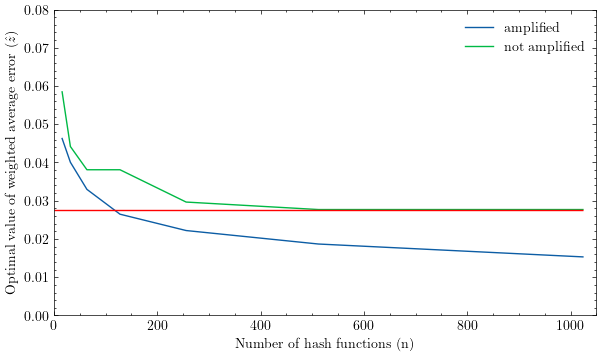
\includegraphics[width=\textwidth]{z_vs_sketch_length_t_02.png}
    \caption[Plot of $\hat{z}$ vs $n$ given $t=0.2$]{\textbf{Plot of $\hat{z}$ vs $n$ given $t=0.2$}. This figure shows the the optimal value $\hat{z}$ of the z-function from Equation \ref{eq:optimization_amplified} for different number of hash functions $n$ and given threshold value = $0.2$. The red line denotes the optimal value of $\hat{z}$ that is achieved for the non-amplified structure}
    \label{fig:z_vs_sketch_length_t_02}
    \end{minipage}
    \hfill 
    \begin{minipage}[b]{0.49\textwidth}
    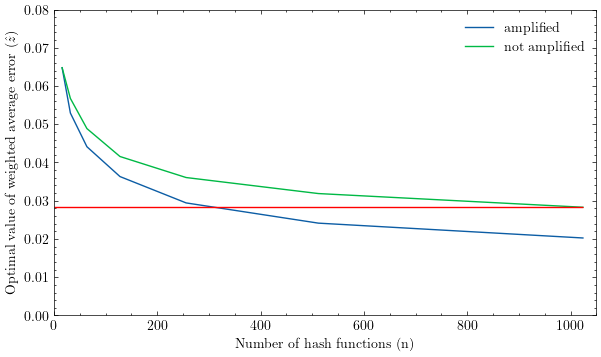
\includegraphics[width=\textwidth]{z_vs_sketch_length_t_06.png}
    \caption[Plot of $\hat{z}$ vs $n$ given $t=0.6$]{\textbf{Plot of $\hat{z}$ vs $n$ given $t=0.6$}. This figure shows the the optimal value $\hat{z}$ of the z-function from Equation \ref{eq:optimization_amplified} for different number of hash functions $n$ and given threshold value = $0.6$.The red line denotes the optimal value of $\hat{z}$ that is achieved for the non-amplified structure}
    \label{fig:z_vs_sketch_length_t_06}
\end{minipage}
\end{figure}

In both figures we draw a horizontal red line at the minimum level of $\hat{z}$ that is achieved for the non-amplified structure. This naturally coincides with the value of $\hat{z}$, where $n=1024$. Special attention can be paid to the level of $n$ where this horizontal red line crosses the green curve. This is the level of $n$ where an amplified scheme shows theoretically equal performance compared to a non-amplified scheme with $n=1024$. For the small threshold $t=0.2$ we observe that this happens at a value of $n$ less than $150$. That is almost $7$ times smaller than $1024$. For $t=0.6$ we find a value of $n$ that is about $4$ times smaller than $1024$, where the non-amplified scheme shows theoretically equal performance compared to a non-amplified scheme with $n=1024$. This highlights that amplified schemes might prove very advantageous in applications where a limited number of hash functions is preferred.

\begin{figure}
    \centering
    \begin{minipage}[b]{0.49\textwidth}
    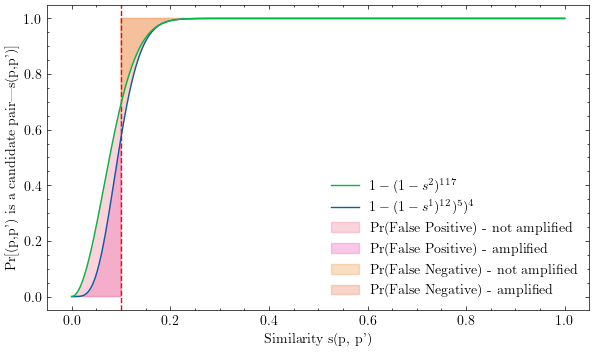
\includegraphics[width=\textwidth]{error_s_curve_t01_n_256.png}
    \caption[Plot of s-curves of (non-)amplified scheme for $t=0.1$ and $n=256$]{\textbf{Plot of s-curves of (non-)amplified scheme for $t=0.1$ and $n=256$}. This figure shows the s-curves for the optimal amplified and non-amplified structure of LSH given that the threshold is $0.1$ and the number of hash functions used is $256$. The sum of the pink and orange areas is equal to $\hat{z}$. }
    \label{fig:error_s_c_curve_t01_256}
    \end{minipage}
    \hfill 
    \begin{minipage}[b]{0.49\textwidth}
    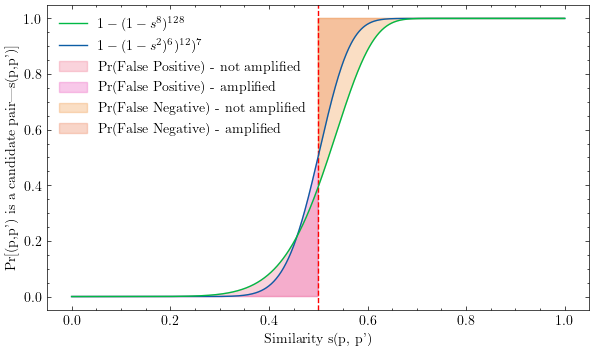
\includegraphics[width=\textwidth]{error_s_curve_t05_n_1024.png}
    \caption[Plot of s-curves of (non-)amplified scheme for $t=0.5$ and $n=1024$]{\textbf{Plot of s-curves of (non-)amplified scheme for $t=0.5$ and $n=1024$}.This figure shows the s-curves for the optimal amplified and non-amplified structure of LSH given that the threshold is $0.5$ and the number of hash functions used is $1024$. The sum of the pink and orange areas is equal to $\hat{z}$. }
    \label{fig:error_s_curve_t05_n_1024}
\end{minipage}
    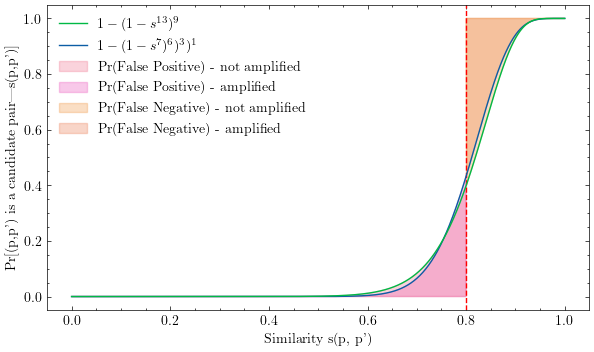
\includegraphics[width=0.49\textwidth]{error_s_curve_t08_n_128.png}
    \caption[Plot of s-curves of (non-)amplified scheme for $t=0.8$ and $n=128$]{\textbf{Plot of s-curves of (non-)amplified scheme for $t=0.8$ and $n=128$}.This figure shows the s-curves for the optimal amplified and non-amplified structure of LSH given that the threshold is $0.8$ and the number of hash functions used is $128$. The sum of the pink and orange areas is equal to $\hat{z}$. }
    \label{fig:error_s_curve_t08_n_128}
\end{figure}

We can also use the form of the s-curve to show potential benefits of amplification. In Figure \ref{fig:error_s_c_curve_t01_256}, \ref{fig:error_s_curve_t05_n_1024}, and \ref{fig:error_s_curve_t08_n_128} we plot the form of the non-amplified and amplified s-curve for different hyperparameter configurations $t$ and $n$. In each figure, we highlight $\operatorname{Pr}[\text{False positive}]$ and $\operatorname{Pr}[\text{False negative}]$. 
One might note the similarity of these graphs to the graph in Figure \ref{fig:change_in_s_curve_as_n_increases}. Indeed, amplification seems to have a comparable effect as an increase of $n$: the form of the s-curve becomes more like a step function. 



\section{Comparing MinHash with FSS}
\label{section:results:MinHash_vs_FSS}

In this section we aim to compare the performance of MinHash with FSS, in order to answer the first research subquestion. 
\begin{figure}
    \centering
    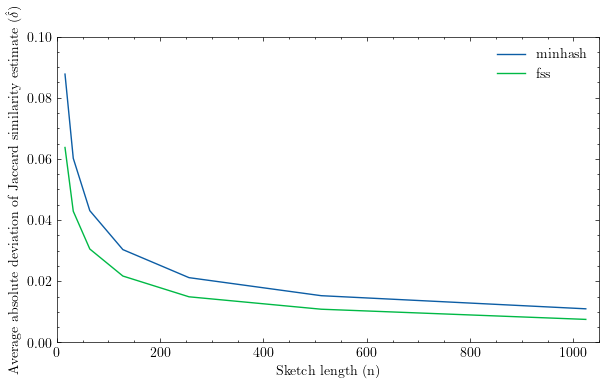
\includegraphics[width=0.75\textwidth]{minhash_vs_fss_preciseness.png}
    \caption[Preciseness of Jaccard similarity estimation of MinHash and FSS for different sketch lengths]{\textbf{Preciseness of Jaccard similarity estimation of MinHash and FSS for different sketch lengths}. The plot shows the average absolute deviation of the estimates of the Jaccard similarity to the true Jaccard similarity of MinHash and FSS for sketch lengths $n\in\{16,32,64,128,256,512,1024\}$. For each sketch length, the reported figure is the result of averaging over the estimates for the $399$ pairwise duplicates in the dataset.}
    \label{fig:minhash_vs_fss_jaccard_estimation_preciseness}
\end{figure}

We first discuss the results of an expirement on the preciseness of Jaccard similarity estimates resulting from MinHash sketches and FSS sketches. The experiment proceeds as follows: for each pairwise duplicate, we generate $10$ pairs of FSS sketches and $10$ pairs of MinHash sketches. Each of these pairs of sketches is then used to estimate the Jaccard similarity. For both sketching methods, we compute the average absolute deviation of the estimated Jaccard similarity from the true Jaccard similarity over the $10$ sketches. We then take the average over the $399$ pairwise duplicates in the dataset to generate an estimate of the absolute deviation $\hat{\delta}$ for each sketching method. We run this experiment for different sketch lengths $n$ as defined in Equation \ref{eq:possible_parameters}. The results of the experiment are shown in Figure \ref{fig:minhash_vs_fss_jaccard_estimation_preciseness}. The plot shows a consistent pattern of MinHash requiring a doubling of the sketch length $n$ to achieve the same value of $\hat{\delta}$. For example, for $n=64$ we find $\hat{\delta}_{FSS} = 0.03054$, while for $n=128$ we have $\hat{\delta}_{MinHash} = 0.03035$. Hence, we can confirm that FSS generates more precise estimates of the Jaccard similarity compared to MinHash. 

Does the increases preciseness of FSS over MinHash also lead to better results in our application of LSH? To answer this question, in the following paragraphs we discuss the result of the bootstrap evaluation as presented in Section \ref{section:meth:evaluation_lsh_schemes}. All reported values in the remainder of this section and the next section are the result of averaging over the bootstrap iterations. 
%In order to provide a concise discussion, we refer to LSH scheme configurations in the following format: $LSH_{MinHash/FSS,A/N,64/128/256/512/1024}$. For example, $LSH_{MinHash,A,256}$ refers to an amplified MinHash LSH scheme with $n=256$, while $LSH_{FSS,N,512}$ refers to a non-amplified FSS LSH scheme with $n=512$.

In Table \ref{table:alpha_max_results} we list the maximum value of $\alpha = PC * RR$ for a wide range of configurations of the LSH scheme. We find that for $n=64$ and $n=128$ FSS is able to achieve considerably higher scores than MinHash for $\alpha_{max}$, both in the amplified and non amplified case. This result is in accordance with our expectations, since we expect that the higher preciseness of FSS sketches compared to MinHash sketches would lead to better results when $n$ is relatively small. For almost all configurations, amplified and non-amplified, FSS delivers better results than MinHash. When MinHash does perform better, e.g. for $n=256$ in the non-amplified setting, the difference with respect to $\alpha_{max}$ between the two sketches is negligible. 
% It is of interest to note that for FSS we find the maximum values of $\alpha$ at a higher threshold ($t=0.20$ or $t=0.25$) than for MinHash ($t=0.15$) when $n$ is small. For values of $n\geq 256$ the maximum value of $\alpha$ is always found at $t=0.15$.

\begin{table}[!htb]
    \centering
    \caption[Bootstrap results]{\textbf{Bootstrap results}. This table lists the bootstrapped results of $\alpha_{max}$, AUC, and $\Delta \%$ AUC  for different configurations of the LSH scheme. We also report the threshold $t$ at which $\alpha$ is maximized and the respective values of PC and RR. Moreover, we report the average time in seconds per bootstrap iteration. The last column contains the specific paramater setting ($r_1,b_1,r_2,b_2$) that is used.}

    \begin{tabular}{|l|l|l|l|l|l|l|l|l|l|l|}
        \hline
        $n$ &  \begin{tabular}{@{}c@{}}Ampl- \\ ified\end{tabular} & \begin{tabular}{@{}c@{}}Sketching \\ Scheme\end{tabular} & $\alpha_{max}$ & $\{t: \alpha_t = \alpha_{max}\}$ & PC & RR & AUC & $\Delta \%$ AUC & Time (s) & ($r_1,b_1,r_2,b_2$) \\
        \hline
        64 &        No &         FSS & 0.7218 &       0.15 &             0.8579 &           0.8413 & 0.4196 &                 - &      2.2525 &  (2,1,32,1) \\
        64 &        No &     MinHash & 0.7038 &       0.15 &             0.8513 &           0.8267 & 0.4151 &                 - &      2.4023 &  (2,1,32,1) \\
        64 &       Yes &         FSS & 0.7382 &       0.15 &             0.9216 &           0.8010 & 0.4312 &          2.7678 &     18.8685 &   (1,3,7,3) \\
        64 &       Yes &     MinHash & 0.7235 &       0.15 &             0.9011 &           0.8029 & 0.4265 &          2.7442 &     18.8654 &   (1,3,7,3) \\
       128 &        No &         FSS & 0.7252 &       0.10 &             0.9418 &           0.7700 & 0.4240 &                 - &      4.1762 &  (2,1,64,1) \\
       128 &        No &     MinHash & 0.7130 &       0.15 &             0.9217 &           0.7736 & 0.4223 &                 - &      3.6497 &  (2,1,51,1) \\
       128 &       Yes &         FSS & 0.7514 &       0.15 &             0.9010 &           0.8340 & 0.4371 &           3.0893 &     35.1595 &   (1,4,6,5) \\
       128 &       Yes &     MinHash & 0.7371 &       0.15 &             0.9026 &           0.8166 & 0.4331 &          2.5516 &     36.7297 &   (1,4,6,5) \\
       256 &        No &         FSS & 0.7298 &       0.15 &             0.9107 &           0.8014 & 0.4288 &                 - &      2.8694 &  (2,1,51,1) \\
       256 &        No &     MinHash & 0.7317 &       0.15 &             0.9277 &           0.7887 & 0.4281 &                 - &      3.4112 &  (2,1,51,1) \\
       256 &       Yes &         FSS & 0.7595 &       0.15 &             0.8948 &           0.8488 & 0.4391 &           2.4124 &     68.7779 &   (1,7,9,4) \\
       256 &       Yes &     MinHash & 0.7475 &       0.15 &             0.8859 &           0.8438 & 0.4377 &          2.2403 &     71.3043 &   (1,7,9,4) \\
       512 &        No &         FSS & 0.7432 &       0.15 &             0.8637 &           0.8605 & 0.4299 &                 - &      2.5025 & (3,1,170,1) \\
       512 &        No &     MinHash & 0.7400 &       0.15 &             0.8664 &           0.8541 & 0.4302 &                 - &      2.7483 & (3,1,170,1) \\
       512 &       Yes &         FSS & 0.7645 &       0.15 &             0.9179 &           0.8329 & 0.4420 &          2.8256 &    138.8113 &   (1,8,9,7) \\
       512 &       Yes &     MinHash & 0.7676 &       0.15 &             0.9136 &           0.8403 & 0.4427 &          2.8974 &    141.3019 &   (1,8,9,7) \\
      1024 &        No &         FSS & 0.7579 &       0.15 &             0.9211 &           0.8228 & 0.4354 &                 - &      3.9461 & (3,1,301,1) \\
      1024 &        No &     MinHash & 0.7428 &       0.15 &             0.9225 &           0.8052 & 0.4325 &                 - &      5.0843 & (3,1,301,1) \\
      1024 &       Yes &         FSS & 0.7745 &       0.15 &             0.9084 &           0.8526 & 0.4455 &          2.3074 &    272.3459 & (1,14,12,6) \\
      1024 &       Yes &     MinHash & 0.7758 &       0.15 &             0.9149 &           0.8479 & 0.4451 &          2.9070 &    281.7397 & (1,14,12,6) \\
      \hline


    \end{tabular}
    \label{table:alpha_max_results}
\end{table}

We can draw the same conclusions graphically. Figure \ref{fig:comparing_minhash_with_fss} shows a plot of the bootstrapped results of the $PC$ and $RR$ for FSS and MinHash for $n=64$ and $n=512$. The dots represent the averaged values per threshold $t$. The ideal method produces values that are in the top-right corner as much as possible, since that would indicate a high value for $PC$, $RR$, and $\alpha$. For $n=128$, the curve of FSS lies more to the right than the curve of MinHash, achieving better results for multiple values of $t$. We notice that for $n=512$, MinHash and FSS achieve almost the same results. In general, the results seems to indicate that FSS is at least as effective as MinHash, with a bigger edge as $n$ becomes smaller. If we also take into account that FSS is a more efficient sketching method for the dataset of interest, as shown in Section \ref{section:data:data_preparation}, then it becomes clear that FSS should be the preferred sketching method.

\begin{figure}
    \centering
    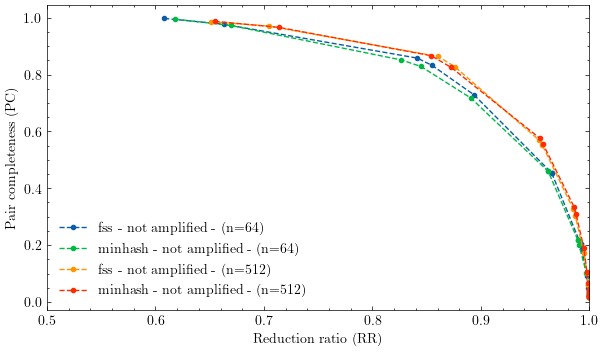
\includegraphics[width=0.75\textwidth]{Comparison of non-amplified MinHash with FSS for n=64,512.png}
    \caption[Comparison of performance of MinHash with FSS]{\textbf{Comparison of performance of MinHash with FSS}.}
    \label{fig:comparing_minhash_with_fss}
\end{figure}

\section{Performance of (amplified) LSH schemes}
\label{section:results:amplified_vs_non_amplified}
In Section \ref{section:results:results_optimization} we have discussed the estimated theoretical benefits of using amplified over non-amplified schemes. In this section we examine the results of amplification applied to the dataset of interest. Table \ref{table:alpha_max_results} contains relevant information. First, we observe that $\alpha_{max}$ is always higher for the amplified configuration than for the non-amplifed configuration, ceteris paribus. We also find evidence that the use of amplification can compensate for a lower value of $n$. For example, for $n=256$, the amplified version of FSS has an almost equal value of $\alpha_{max}$ as the non-amplified version of FSS for $n=1024$. For MinHash, the amplified version for $n=256$ even surpasses the non-amplified version for $n=1024$ with respect to $\alpha_{max}$. %This is mostly driven by a decrease of $\operatorname{Pr}[\text{False positive}]$, since we observe that amplification is associated with relatively large increases of $RR$, while $PC$ stays constant or decreases by a relatively small amount.   
% Based on the results from section \ref{section:results _optimization}, we would expect amplified LSH schemes to perform relatively stronger as the number of hash functions $n$ increases.
\begin{figure}
    \centering
    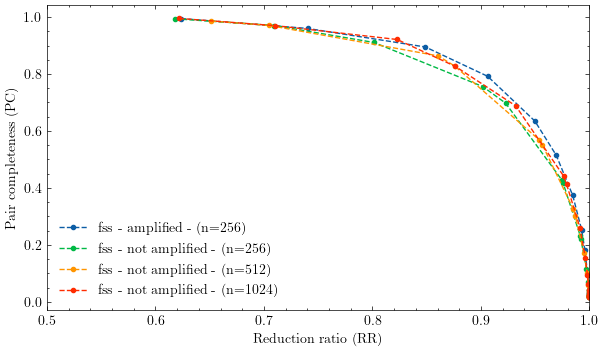
\includegraphics[width=0.75\textwidth]{increase_n_vs_amplified_effect.png}
    \caption[Plot of PC and RR for different configurations of MinHash]{\textbf{Plot of PC and RR for different configurations of MinHash}}
    \label{fig:effect_of_n_vs_amplification}
\end{figure}
Figure \ref{fig:effect_of_n_vs_amplification} contains a plot of the $PC$ and $RR$. We include $3$ non-amplified FSS schemes with $n=256$, $n=512$ and $n=1024$. As $n$ increases, the curve moves outwards to the right: an increase of $n$ is associated with higher values of $RR$ and $PC$. We also add the curve (in blue) related to the amplified FSS scheme with $n=256$ to the plot. This curve lies clearly to the right of the non-amplified $n=256$ and $n=512$ FSS curves, while following about the same path as the non-amplified $n=1024$ FSS curve. This adds more substance to the argument that amplification can compensate for using a smaller number of hash functions. 

\begin{figure}[!htb]
    \centering
    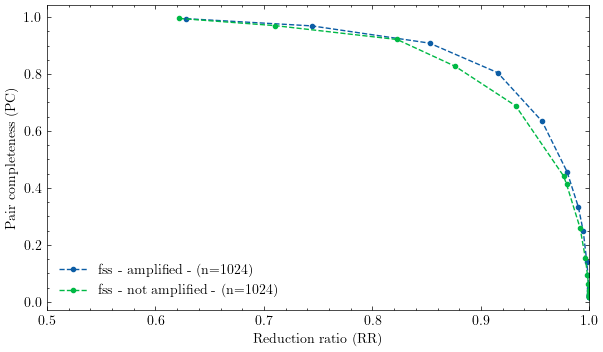
\includegraphics[width=0.75\textwidth]{minhash_amplified_vs_non_amplified_1024.png}
    \caption[Effect of amplification on $PC$ and $RR$ for FSS scheme with $n=1024$]{\textbf{Effect of amplification on $PC$ and $RR$ for FSS scheme with $n=1024$}}
    \label{fig:Effect of amplification - minhash}
\end{figure}
This is also confirmed by an inspection of the \textit{area under the curve} ($AUC$) of the $PC$ and $RR$ plot for the different configurations, which can also be found in Table \ref{table:alpha_max_results}. We use the trapezoid rule to estimate the $AUC$ on a range of $RR\in[0.5,1]$, assuming that a $RR$ of $0.5$ would lead to a $PC$ of 1. We deem this a valid assumption, since a $RR$ of circa $0.6$ is already associated with a $PC>0.99$ for all methods tested. The theoretically ideal value of $AUC$ is $0.5$, which would be the case if $PC$ and $RR$ are $1$ for a certain configuration. %The values of $AUC$ are quite close to $1$, since for a large part of the range of $RR$ we obtain $PC$ values of almost $1$. 
The column titled $\Delta \%$ AUC in Table \ref{table:alpha_max_results} shows the increase in percentage of the $AUC$ score of the amplified scheme compared to the corresponding non-amplified scheme. In general, we find substantial increases of $AUC$ as a result of amplification for all configurations.

Focusing on a single value of $n$, for example $n=1024$, we find strong evidence for a positive effect of amplification on the effectiveness of LSH as well. We present Figure \ref{fig:Effect of amplification - minhash}, which shows the $PC$-$RR$ curve for the amplified and non-amplified FSS scheme with $n=1024$. The main conclusion to draw from the plot is that for every value of $PC$ that a user might aim for in an application, the amplified scheme is able to deliver such a value paired with a higher RR. Similar plots for smaller values of $n$ can be found in Appendix \ref{appendix:plots_effect_amplification}.

When it comes to efficiency, the results confirm the suspicisions as laid out in Section \ref{section:results:results_optimization}. We observe in Table \ref{table:alpha_max_results} that smaller values for $r_1$ are indeed associated with a less efficient LSH scheme. As $n$ increases, the optimal value of $r_1$ increases for the non-amplified LSH schemes. For the amplified LSH schemes the optimal value is still equal to $1$. This leads to increased differences in efficiency as $n$ increases between the most effective amplified and non-amplified LSH schemes. For $n=64$, the most effective amplified LSH scheme takes around 7 times as more time than the most effective non-amplified LSH scheme. For $n=1024$, this factor has increased to as much as 60. If one would require a more efficient amplified scheme, then one could implement restrictions on the parameter $r_1$ when optimizing the paramater configuration. This would come down to choosing a value for $r_1$ that is higher than $1$, but still smaller than the value of $r_1$ in the non-amplified scheme. For $n=1024$, one could for example let $r_1=2$ and choose $r_2$, $b_1$ and $b_2$ such that the function $z(r_1,b_1,r_2,b_2| w_{FP}, w_{FN})))$ in Equation \ref{eq:optimization_amplified} is minimized.

% Based on early evaluation results, we seem to be able to confirm this suspicion. In figure \ref{fig:no_perm_64_pc_rr} we plot the PC vs the RR for $n=64$. On a large area of the graph, the non-amplified MinHash scheme performs as well as its amplified counterpart. In figure \ref{fig:no_perm_256_pc_rr} we find that for a fairly large range of reduction ratio's both amplified hashing schemes achieve a higher PC for the same RR. 

% A second observation one can make is that especially in the non-amplified case MinHash seems to be outperforming FSS. In section \ref{section:MinHash_vs_FSS} we take a closer look at possible reasons.

% \begin{figure}[h!]
%     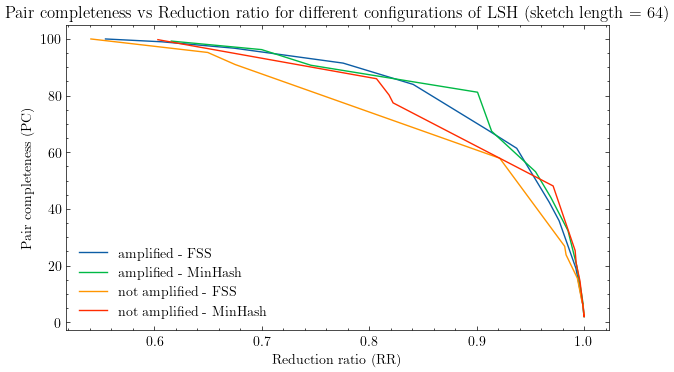
\includegraphics[width=\textwidth]{no_perm_64_pc_rr.png}
%     \caption{Plot of pair completeness (PC) vs reduction ratio (RR). Number of hash functions used is 64.}
%     \label{fig:no_perm_64_pc_rr}
% \end{figure}

% \begin{figure}[h!]
%     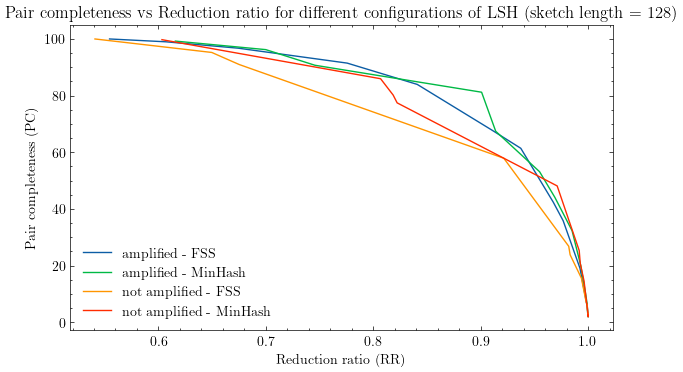
\includegraphics[width=\textwidth]{no_perm_128_pc_rr.png}
%     \caption{Plot of pair completeness (PC) vs reduction ratio (RR). Number of hash functions used is 128.}
%     \label{fig:no_perm_128_pc_rr}
% \end{figure}

% \begin{figure}[h!]
%     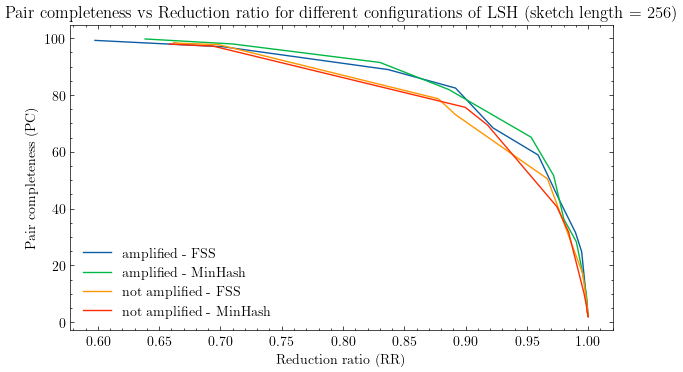
\includegraphics[width=\textwidth]{no_perm_256_pc_rr.png}
%     \caption{Plot of pair completeness (PC) vs reduction ratio (RR). Number of hash functions used is 256.}
%     \label{fig:no_perm_256_pc_rr}
% \end{figure}

% Note: I still need to evaluate this graph for n=512 and n=1024, but I first need to improve the speed of candidate extraction of the amplified LSH scheme. One option is to set some constraints  This will also help with the efficiently running the bootstrap evaluation.